\documentclass[12pt]{article}

\usepackage{graphicx}
\usepackage{url}
\usepackage{color}
\usepackage{fancyhdr}
\usepackage[T1]{fontenc}
\usepackage[polish]{babel}
\usepackage[utf8]{inputenc}
\usepackage{lmodern}
\usepackage{caption}
\usepackage{listings}
\selectlanguage{polish}
\title{My first document}
\author{Kamil Warpechowski}



\fancypagestyle{firststyle}
{
   \fancyhf{}
   \fancyfoot[C]{
		Warszawa, \today
   }
}

\usepackage{color}
\definecolor{bluekeywords}{rgb}{0.13,0.13,1}
\definecolor{greencomments}{rgb}{0,0.5,0}
\definecolor{redstrings}{rgb}{0.9,0,0}

\lstdefinelanguage{CSharp}
{
 morecomment = [l]{//}, 
 morecomment = [l]{///},
 morecomment = [s]{/*}{*/},
 morestring=[b]", 
 sensitive = true,
 morekeywords = {abstract,  event,  new,  struct,
   as,  explicit,  null,  switch,
   base,  extern,  object,  this,
   bool,  false,  operator,  throw,
   break,  finally,  out,  true,
   byte,  fixed,  override,  try,
   case,  float,  params,  typeof,
   catch,  for,  private,  uint,
   char,  foreach,  protected,  ulong,
   checked,  goto,  public,  unchecked,
   class,  if,  readonly,  unsafe,
   const,  implicit,  ref,  ushort,
   continue,  in,  return,  using,
   decimal,  int,  sbyte,  virtual,
   default,  interface,  sealed,  volatile,
   delegate,  internal,  short,  void,
   do,  is,  sizeof,  while,
   double,  lock,  stackalloc,   
   else,  long,  static,   
   enum,  namespace,  string}
}


\lstset{,
  showspaces=false,
  showtabs=false,
  breaklines=true,
  showstringspaces=false,
  breakatwhitespace=true,
  escapeinside={(*@}{@*)},
  frame=lrtb,
  aboveskip=2em
}

\setlength{\parindent}{1em}
\begin{document}


\thispagestyle{firststyle}
\begin{center}

\includegraphics[width=1\textwidth]{images/logo.jpg}
\textbf{Wydzial Informatyki} \\
\vspace{3em}
\textbf{Katedra Sieci Komputerowych} \\
Sieci Urządzeń Moblinych \\
\vspace{3em}
\textbf{Kamil Warpechowski} \\
Nr albumu 10709
\end{center}


\vspace{3em}
{\addtolength{\leftskip}{70mm}

\noindent
Praca inżynierska
\\Promotor:
\\dr inż. Michał Tomaszewski

}

\vspace{3em}

\textbf {
	tutaj będzie zajebisty tytuł
}

\newpage
\tableofcontents
\newpage
  
\section{Wprowadzenie}
\paragraph{}
Ludzie od lat przyzwyczaili się korzystać z elektroniki oraz internetu na standardowych urządzeniach elektronicznych. Na początku lat dziewiędziesiątych do domów zaczęły trafiać komputery stacjonarne. Najpierw z modemami DLS, a następnie już ze stałymi łączami. Na przestrzeni lat korzystanie z ekranu w połączeniu z klawiaturą i myszą stało się dla ludzi naturalne.

Przez ostatnią dekadę na rynku pojawiły się interfejsy dotykowe. Popularność smartfonów, a następnie tabletów spowodowało, że coraz bardziej sporadyznie korzystamy z standardowej fizycznej klawiatury.
Ekrany dotykowe pojawiły się nie tylko na urządzeniach telekomunikacyjnych, lecz także jako moniotory w komputerach pokładowych samochodów oraz instalowane są w zagłówkach w samolotach jako multimedialne centrum rozrywki {\footnote{http://www.komputerswiat.pl/nowosci/wydarzenia/2012/28/boeing-z-androidem-na-pokladzie.aspx}).
\paragraph{}
Przez ostatnie kilka lat narasta trend poszukiwania innych metod dostępu do danych, zwłaszcza multimedialnych. Obecnie wiele przedsiębiorstw prowadzi badania nad nowymi, bardziej naturalnymi interfejsami, które nie wymagałyby użycia standarodwych urządzeń typu klawiatura czy myszka.

Wiele nowych urządzeń próbuje implementować sterowanie intefejsem użytkownika za pomocą gestów (np. Microsoft Kinect\footnote{http://www.xbox.com/pl-PL/xbox-one/accessories/kinect-for-xbox-one}), czy też za pomocą myśli (np. Emotiv {\footnote{http://emotiv.com}). Na rynku widać duże zainteresowanie nową formą kontroli urządzeniami, zwłaszcza tymi bardziej naturalnymi dla człowieka.

\paragraph{}
{\color{red}Natural UI interface - tutaj dopisać}

\begin{center}
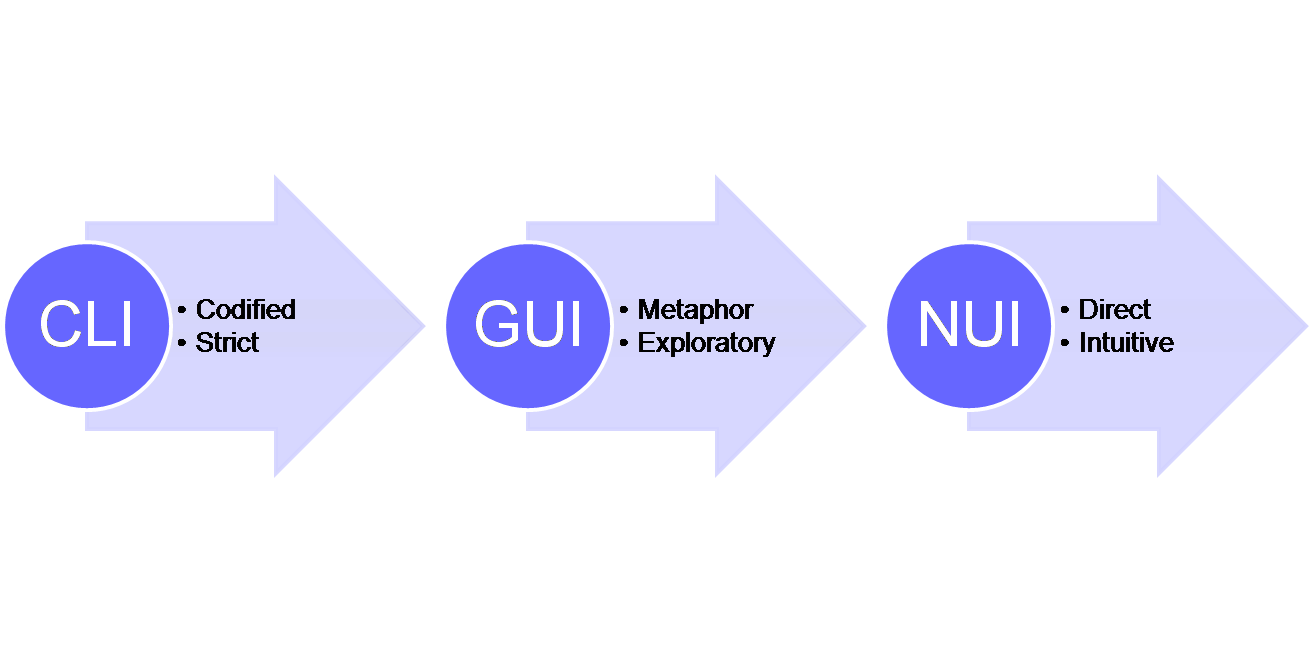
\includegraphics[width=0.9\textwidth]{images/nui.png}
\captionof{figure}{
Ewolucja interfejsów użytkownika
}
\small {źródło: https://en.wikipedia.org/wiki/Natural_user_interface }
\end{center}

\paragraph{}
W branży filmowej oraz gier wideo narasta trend używania nowych technologii do rozszerzania doznań jakie otrzymuje odbiorca.
W kinach odbywają są coraz częściej projekcje filmów 3D. Natomiast w ostatnim czasie pojawią się sale kinowe pozwaljące  na projecję filmów trójwymiarowych wraz z dodatkowymi elementami takimi jak: drganie foteli, wiatr, dym, woda \footnote{http://cinema-city.pl/4dx-info}. Jednakże w obecnej chwili taki format rozrywki jest dość drogi, gdyż wymaga specjalnie przygotowanej sali kinowej oraz okularów, które pozwalają tworzyć iluzję przestrzenną. 

\subsection{Rozszerzona rzeczywistość}
Coraz bardziej popularne staje się pojęcie rozszerzonej rzeczywistości (ang. augmented reality)

\paragraph{}
Natural Machines, Meta2, Wonderbook
\begin{center}
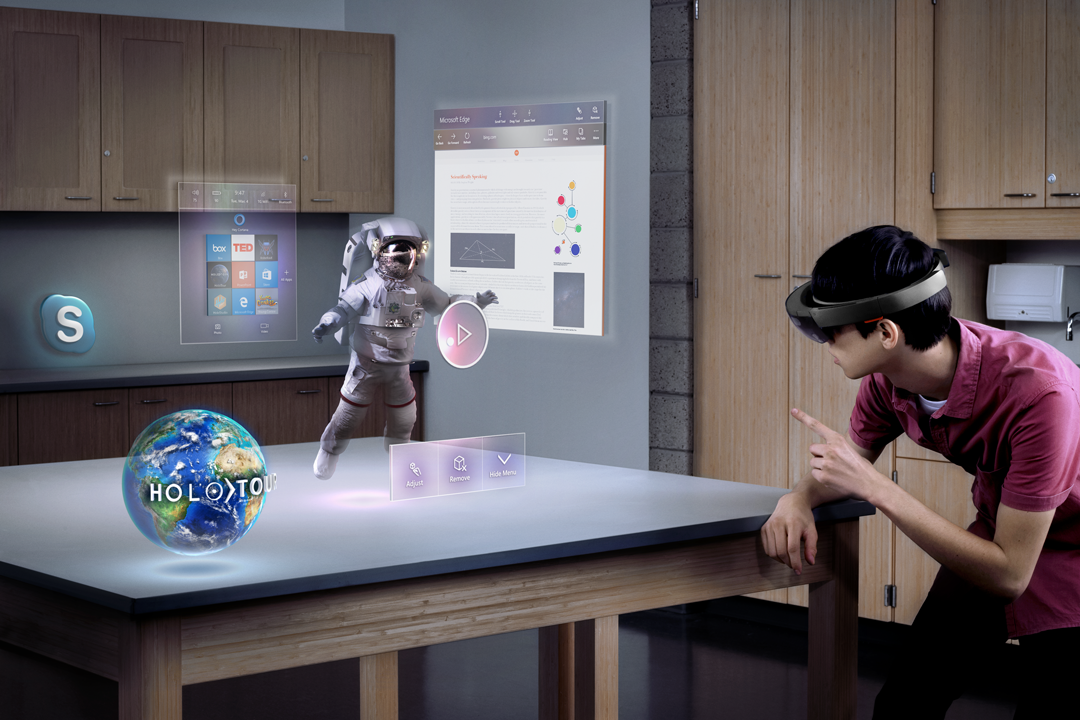
\includegraphics[width=0.9\textwidth]{images/hololens.png}
\captionof{figure}{
Wizualizacja Microsoft HoloLens
}
\small {źródło: https://www.microsoft.com/microsoft-hololens/en-us/why-hololens }
\end{center}


\section{Cel pracy}
\paragraph{}
Celem niniejszej pracy jest stworzenie platformy do budowania gier oraz interaktywnych animacji prezentowanej za pomocą rozszerzonej rzeczywistości sterowaniej za pomocą zdalnego kontrolera.

\paragraph{}
Przykłady zastosowanie zestawu aplikacji:

\begin{itemize}
\item Prezentacje przestrzeni architektonicznych
\item Rozrywka
\item Reklama miejscach użyteczności publicznych (np. centra handlowe)
\end{itemize}


\section{Implementacje}
\subsection{Implementacja w technologii hologramu}
\paragraph{}
{\color{red}Tutaj opisać próby i przemyślenia na temat hologramu na drzwiach.}
\begin{center}
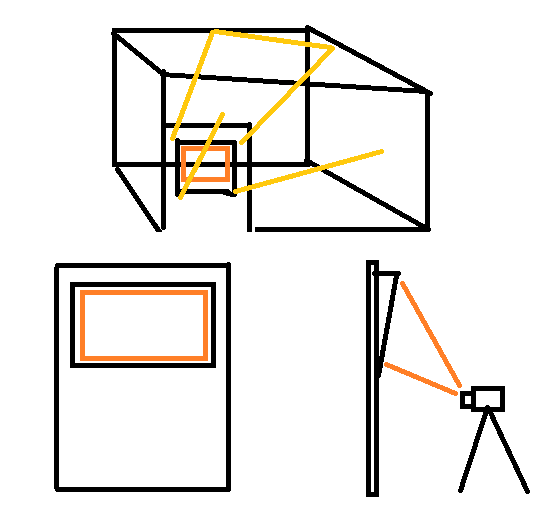
\includegraphics[width=0.9\textwidth]{images/hologramv1.png}
\captionof{figure}{
Poglądowy schemat działania
}
\small {źródło: własne }
\end{center}

\subsection{Implementacja w technologii mappingu 3d}
{\color{red}Tutaj opisać próby i przemyślenia}

\section{Wykorzystane technologie}

\subsection{Unity}
\paragraph{}
Unity jest obecnie najpopularniejszą platformą do tworzenia gier na wiele platform. 
\subsubsection{Dlaczego Unity}
\paragraph{}
Najnowsza wersja posiada natywne wsparcie do rozszerzonej oraz wirtualnej rzeczywistości. Narzędzie te posiada prosty, ergonomiczny interfejs co ułatwia pracę.
\paragraph{}
Bardzo pomocnym dodatkiem do narzędzia jest ,,Assets Store''. Jest to wirtualny sklep z komonentami do tworzenia gry. W projekcie zastosowałem tekstury i obiekty 3D pochodzące z tego źródła.
\subsubsection{Alternatywne rozwiązania}
 \begin{tabular}{|c|c|c|}
 \hline
 \ & Unity & Unreal Engine \\ 
  \hline
 Wsparcie języków programowania & C\#, JavaScript, Boo & c++ \\  
  \hline
 Obsługa wielu ekranów & Tak & Nie \\
 \hline  
  Wsparcie dla Google Cardboard & Tak & Nie \\
  \hline   
  &  &  \\
  \hline   
  &  &  \\
  \hline   
\end{tabular}
\captionof{table}{Porównanie silników gier}

\subsubsection{Wybór języka programowania}
\paragraph{}
Środowisko Unity wspiera obsługę skryptów (animacje oraz logika biznesowa) w kilku językach programowania: C\#, UnityScript (zmodyfikowana wersja JavaScript)  oraz w przeszłości Boo. Podjęto decyzję, by w projekcie użyć język C\#, gdyż ów język jest najbardziej stabilny, posiada najbardziej rozbudowaną dokumentację oraz jest to najpopularniejszy język w specjalistycznej literaturze. Dodatkowym udogodnieniem  jest to, iż  język posiada wiele wbudowanych klas (np. do obsługi połączęń TCP) oraz niezliczoną ilość zewnętrznych bibliotek.
\subsubsection{Unity IDE}
\paragraph{}
Środowisko Unity jest multiplatformowe. Aplikacje można używać na dowolnym sytemie operacyjnym. Jednakże edycja skryptów odbywa się za pomocą zewnętrznego narzędzia. W systemie Mac OS X jest to MonoDevelop, natomiast w systemie Windows jest to VisualStudio w wersji Community. Opisywana aplikacja początkowo była tworzona na systemie Mac OS X, jednakże kołopoty ze środowiskiem MonoDevelop spowodwały decyzje o przeniesieniu środowiska na system Windows. Subiektywnie mogę stwierdzić, że stabilność oraz komfort pracy jest dużo lepszy w systemie Windows.
Dodatkową alternatywą dla MonoDevelop może okazać się Visual Studio Code. Jest to prosty multiplatformowy edytor posiadający obsługę języka C\# .

\subsubsection{Licencja i koszty}
\paragraph{}
Unity jest zamkniętym, licencjonowanym oprogramowaniem. Darmowa wersja (Personal Editon) pozwala na nielimitowane użycie, jednakże jest to okrojona edycja. Szersze informacje o ograniczeniach wersji Personal zawarte są w kolejnych rozdziałach. Licencja pozwala na komercyjne użycie przy limicie zarobków na poziomie stu tysięcy dolarów.
Komercyjna wersja (Professional Edition) jest płatna w modelu subskrybcyjnym (75 dolarów za miesiąc)\footnote{https://store.unity3d.com/subscribe}.
Na potrzeby opisywanego projektu zasotosowano Unity w wersji Personal Edition.

\subsection{Android}
\paragraph{}
Naturalnym wyborem technologii przy tworzeniu aplikacji na urządzenie sterujące byłoby Unity, gdyż te środowisko pozwala na kompilacje kodu na urządzenia mobilne(systemy: iOS, Android, Windows Phone, Tizen itp\footnote{https://unity3d.com/unity/multiplatform}). Jednakże Unity w wersji Personal Edition nie pozwala na uruchomienie warstwy sieciowej na urządzeniach mobilnych.
\paragraph{}
Na potrzeby implementacji przykładowego urządzenia sterującego wybrano platformę Android, gdyż ma ona największy udzła w rynku.\footnote{https://www.netmarketshare.com/operating-system-market-share.aspx?qprid=10&qpcustomd=1} Proces tworzania aplikacji na tą platformę przebiega w języku Java.

\subsubsection{Android Studio}
\paragraph{}
opisac

\subsubsection{Zależności}
\begin{enumerate}
	\item Butter Knife
\end{enumerate}

\subsection{Komunikacja sieciowa}
\paragraph{}
Największym wyzwaniem było stworzenie dwukierunkowego protokołu komunikacyjnego pomiędzy serwerem (aplikacja napisana w środowisku Unity) oraz dowolnym kontrolerem lub w przyszłości innym urządzeniem wysłającym dane do aplikacji. Podstawowym założeniem było to iż, kontrolerem gry może być standardowy telefon komórkowy. Dodatkowo w przyszłości planowana jest rozbudowa o zdalne sterowanie za pomocą przeglądarki internetowej. Pierwotnie ozważane było użycie Bluetooth, jednak ograniczyłoby to zdalne sterowanie. Podjęto decyzję projektową o użyciu połączenia sieciowego. Rozważano następujące protokoły:

\subsubsection{UNET}
\paragraph{}
Unity wspiera natywną obsługę multiplayer - UNET, jednakże jest to zamknięty protokół. Komunikacja możliwa jest tylko pomiędzy aplikacjami stworzonymi w tym środowisku.

\subsubsection{HTTP (SOAP, REST)}
\paragraph{}
Komunikacja za pomocą HTTP (protokoły komunikacyjne takie jak np. SOAP, REST) są bardzo często spotykane. Jest to standard aplikacji internetowych. HTTP nadaje się do przesyłu dużych wolumenów danych, jednak niezbyt dobrze sprawdza się przy małych, lecz częstych połązeniach pomiędzy klientem, a serwerem. Duży narzut czasowy może spowodować transormacja danych do oraz z formatu JSON lub XML. Jednakże dużą zaletą wspomnianych protokołów jest prostota implementacji w większości języków programowania, gdyż są już gotowe komponenty.
\subsubsection{TCP}
\paragraph{}
{\color{red}Opisać, że TCP jest ogólnie lepsze - socket, ale to jest nadal połączeniowy, więc lepiej by było udp}
\subsubsection{UDP}
\paragraph{}
{\color{red}opisać, ze to najlepsze rozwiazanie - bezpolazeniowe}

\newpage
\section{Aplikacja główna}


{\color{red}tutaj będą makiety}

\subsection{Świat gry}
\subsection{Aktorzy}

\begin{center}

 \begin{tabular}{|c|c|}
 \hline  
  &   \\
  \hline   
  &   \\
  \hline   
\end{tabular}
\captionof{table}{Właściwości aktora}
\end{center}

\begin{lstlisting}[language=CSharp]
public void SendInfo() {
	Network.SendMessage("hasax_"+this.hasAx);
	Network.SendMessage("hassh_"+this.hasSh);
	Network.SendMessage("hasdrabina_"+this.drabina);
	Network.SendMessage("isMove_"+this.isMove);
}
\end{lstlisting}
\captionof{lstlisting}{
	Do Poprawy
}

\subsection{Kamery}
\paragraph{}
Platforma Unity wspiera do 8 wirtualnych kamer \footnote{http://docs.unity3d.com/Manual/MultiDisplay.html}.
Każda z tych kamer może być prezentowana na oddzielnym fizycznym ekranie.

\subsection{Prefabrykaty}
\paragraph{}
W Unity możliwe jest używanie prefabrykatów (Prefabs \footnote{http://docs.unity3d.com/Manual/Prefabs.html}). Są obiekty lub grupy obiektów, które służą do wielokrotnego wykorzystywania. W Projekcie założono, że wszystkie reużwalne komponety (dziedziczone pomiędzy scenami) będą prefabrykatami.

Dodatkowo aktorzy gry (generowane dynamicznie) są również prefabrykatami. Instancje aktora są tworzone podczas działania aplikacji.

{\color{red}Opisać prefabrykaty}

\subsection{Logika biznesowa}
\subsection{Serwer komunikacyjny}
\newpage
\section{Aplikacja mobilna - kontroler}

\begin{center}
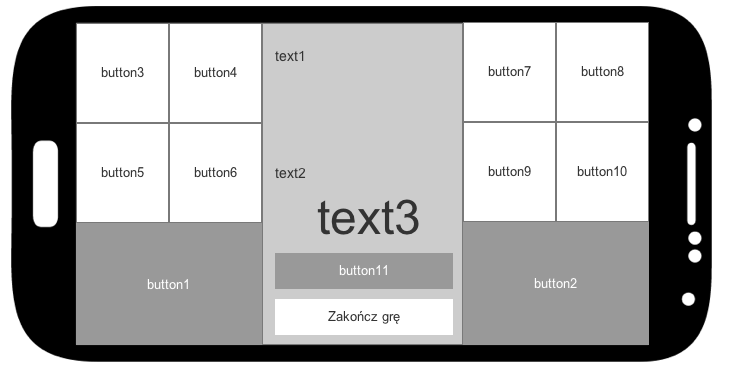
\includegraphics[width=1\textwidth]{images/button_mockup.png}
\captionof{figure}{
Makieta - układ przycisków
}
\end{center}
\paragraph{}
Głównym założeniem było stworzenie uniwersalnego kontrolera przygotowanego pod dowolny rodzaj gry, bądź innej wizualizacji stworzonej w środowisku Unity. Podczas uruchomienia kontrolera serwer wysyła statusy przycisków oraz pól tekstowych.

\subsection{Przyciski}
\paragraph{}
Każdy przycisk może zostać skonfigurowany poprez ustawienie tekstu. Dodatkowo można zablokować przycisk podczas gdy nie jest on potrzebny w danym czasie.
\paragraph{}
Aby ułatwić pracę nad aplikacją stworzono pole wyliczalne (ENUM) zawierającą wszystkie przyciski.

\begin{lstlisting}[language=Java]
public enum ButtonEnum {
    BTN1, BTN2, BTN3, BTN4, BTN5, BTN6, BTN7, BTN8, BTN9, BTN10, BTN11
}
\end{lstlisting}
\captionof{lstlisting}{
	Enum z przyciskami
}
\paragraph{}
Jednakże aby powiązać elementy ,,Button'' z warstwy widoku (defincja XML) na kod przycisku  należy stworzyć listę elementów. Będzie ona służyła do wyszukiwania przycisków oraz zmiany ich właściwości. Dodatkowo do każdego przycisku należy dodać obsługę zdarzeń. Po kliknięciu wysyłany będzie odpowiedni komunikat.

\begin{lstlisting}[language=Java]
    protected HashMap<ButtonEnum, Button> buttonsMap = new HashMap<ButtonEnum, Button>();

    protected void mapButton(int btnId, final ButtonEnum btnName) {
        final Button button = (Button) findViewById(btnId);
        buttonsMap.put(btnName, button);

        button.setOnClickListener(new View.OnClickListener() {
            public void onClick(View v) {
                sendToServer("button_" + btnName);
            }
        });
    }
\end{lstlisting}
\captionof{lstlisting}{
	Metoda obsługująca przycisk
}


\begin{lstlisting}[language=Java]
 @Override
    protected void onCreate(Bundle savedInstanceState) {
        super.onCreate(savedInstanceState);

        this.mapButton(R.id.button1, ButtonEnum.BTN1);
        this.mapButton(R.id.button2, ButtonEnum.BTN2);

    }
\end{lstlisting}
\captionof{lstlisting}{
	Przykład mapowania przycisku
}

\subsection{Informacje tekstowe}
\paragraph{}
Pola tekstowe mogą mieć ustawioną dowolną treść w dowolnym czasie.

\subsection{Komunikacja sieciowa}



\section{Środowisko uruchomieniowe}
\paragraph{}
Powyżej opisana aplikacja została uruchomiona testowo w labolatorium na Polsko-Japońskiej Akademii Technik Komputerowych.

\subsection{Serwer}
\paragraph{}
Serwer został uruchomiony na komputerze przenośnym(laptop) posiadającym kartę graficzną umożliwiajacą podłączenie dwóch zewnętrznych ekranów - projektorów. Pierwszy z nich został połączony za pomocą złącza cyfrowego HDMI, natomiast drugi łączem DVI.
\subsection{Aplikacja mobilna - kontroler}


\newpage
\section{Implementacja na platformie Google Cardboard}
\paragraph{}
Innym przykładem implementacji projektu w rozszerzonej rzeczywistości może być platforma Google Cardboard \footnote{https://vr.google.com/cardboard/index.html}. Są to niskobudżetowe okulary stworzone przez firmę Google do wyświetlania wirtualnej rzeczywistości. Kartonowe okulary powstawły w celu wyświetlania obrazu stereoskopowego. Posiadają one miejsce do umieszczenia dowolnego telefonu komórkowego typu smartphone. Do projektu wybrano wersję, która pozwala na umieszczenie telefonu w sposób taki, iż tylna kamera nie jest załonięta przez obudowę. Dzięki temu można użyć platformę Cardboard przeznaczoną pierwotnie tylko do wirtualnej rzeczywistości do stworzenia aplikacji wykorzystującą augmented reality.

\begin{center}
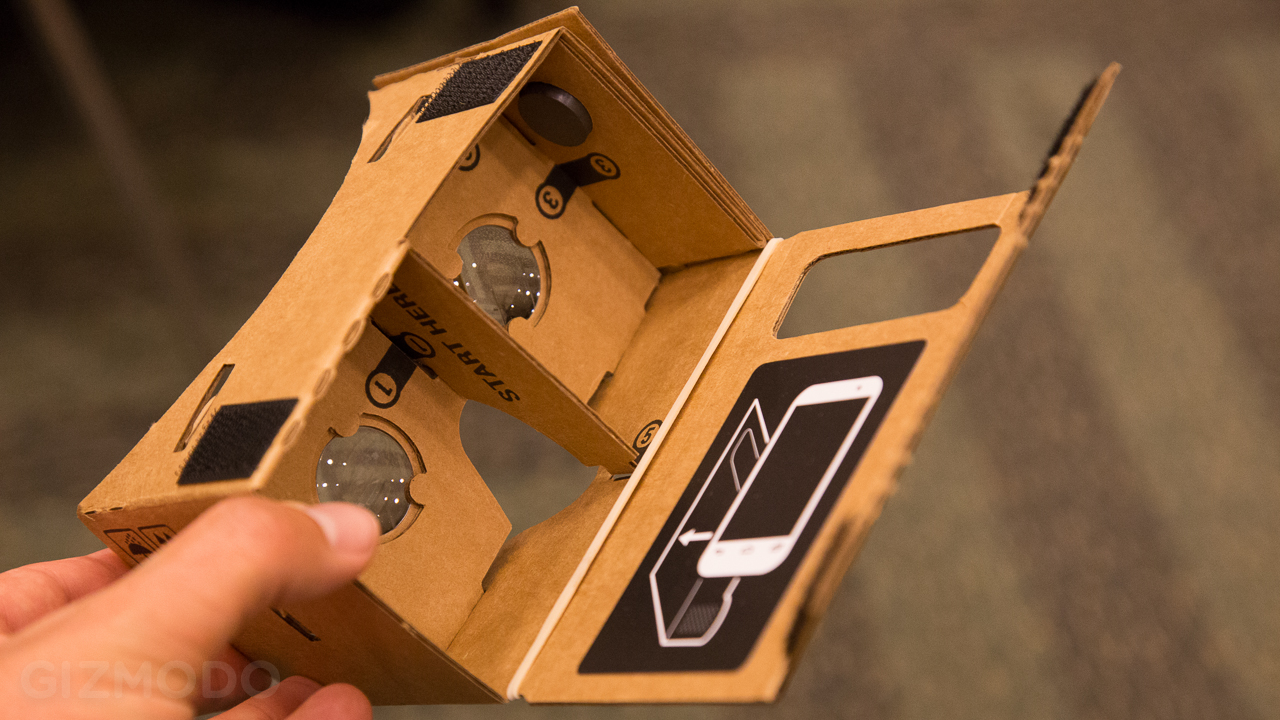
\includegraphics[width=0.9\textwidth]{images/cardboard.jpg}
\captionof{figure}{
Google Cardboard w wersji do samodzielnego złożenia
}
\small {źródło: http://gizmodo.com/turn-your-android-into-a-virtual-reality-headset-with-g-1596026538 }
\end{center}

\paragraph{}
Dzięki użyciu kamery użytkownik widzi obraz znajdujący się przed nim. Aby obraz był stereoskopowy należało stworzyć aplikację, która wyświetlić strumień danych z kamery dzieląc go na dwa obrazy (kolejno dla lewego oraz prawego oka).

\begin{center}
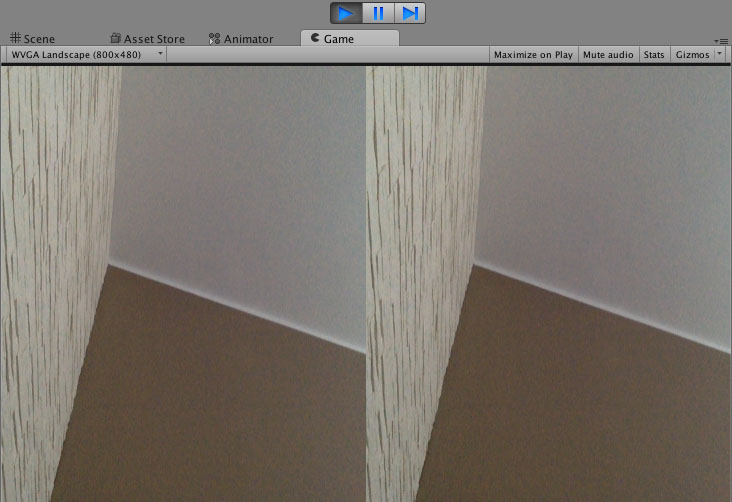
\includegraphics[width=0.9\textwidth]{images/kadr.jpg}
\captionof{figure}{
Ujęcie z kamery aparatu w obrazie stereoskopowym - scena w Unity
}
\small {źródło własne}
\end{center}

\subsection{ArToolkit}
\paragraph{}
W celu wyświetlenia wirtualnych obiektów na obrazie z kamery rozbudowano aplikację z rodziału pierwszego {\color{red}uzupełić rozdział}. Do platformy Unity doinstalowano zewnętrzny komponent ARToolKit  \footnote{http://artoolkit.org/}. Jest to biblioteka wydana przez University of Washington \footnote{https://www.hitl.washington.edu/artoolkit/}, lecz obecnie upostępniona jest na licencji GNU. Kod źródłowy jest otwarty i rozwijany przez środowisko Open Source \footnote{https://github.com/artoolkit}.
\subsection{Markery}
\paragraph{}
Za pomocą tej biblioteki możliwe jest wykrywanie w obrazie z kamery markerów, czyli specjalnie przygotowanych czarno-białych obrazków (w naiwnej implementacji - wydrukowanych na kartkach), oraz nakładanie w ich miejsce trójwymiarowych modeli lub całych scen. Dzięki bibliotece ArToolkit możliwe jest diagnozowanie pod jakim kątem padania oraz w jakiej odległości od urządzenia znajduje się marker. Umiejscowienie tagu analizowane jest w czasie rzeczywistym, co zapewni ciągłą korekcję ułożenia wirtualnych modeli względem ich realnych odpowiedników.

\begin{center}
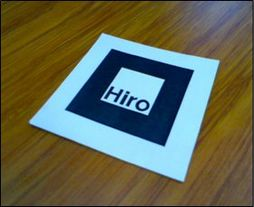
\includegraphics[width=0.9\textwidth]{images/hiro.png}
\captionof{figure}{
Przykład przygotowanego obrazka do rozpoznawania - marker
}

\end{center}
\paragraph{}
Szablony markerów można wykonywać we własnym zakresie. Aby zaimportować nowe obrazki do biblioteki ArToolkit należy przygotować specjalny plik binarny reprezentujący model markera.
\footnote{http://bit.ly/1YU199f}.

\begin{center}
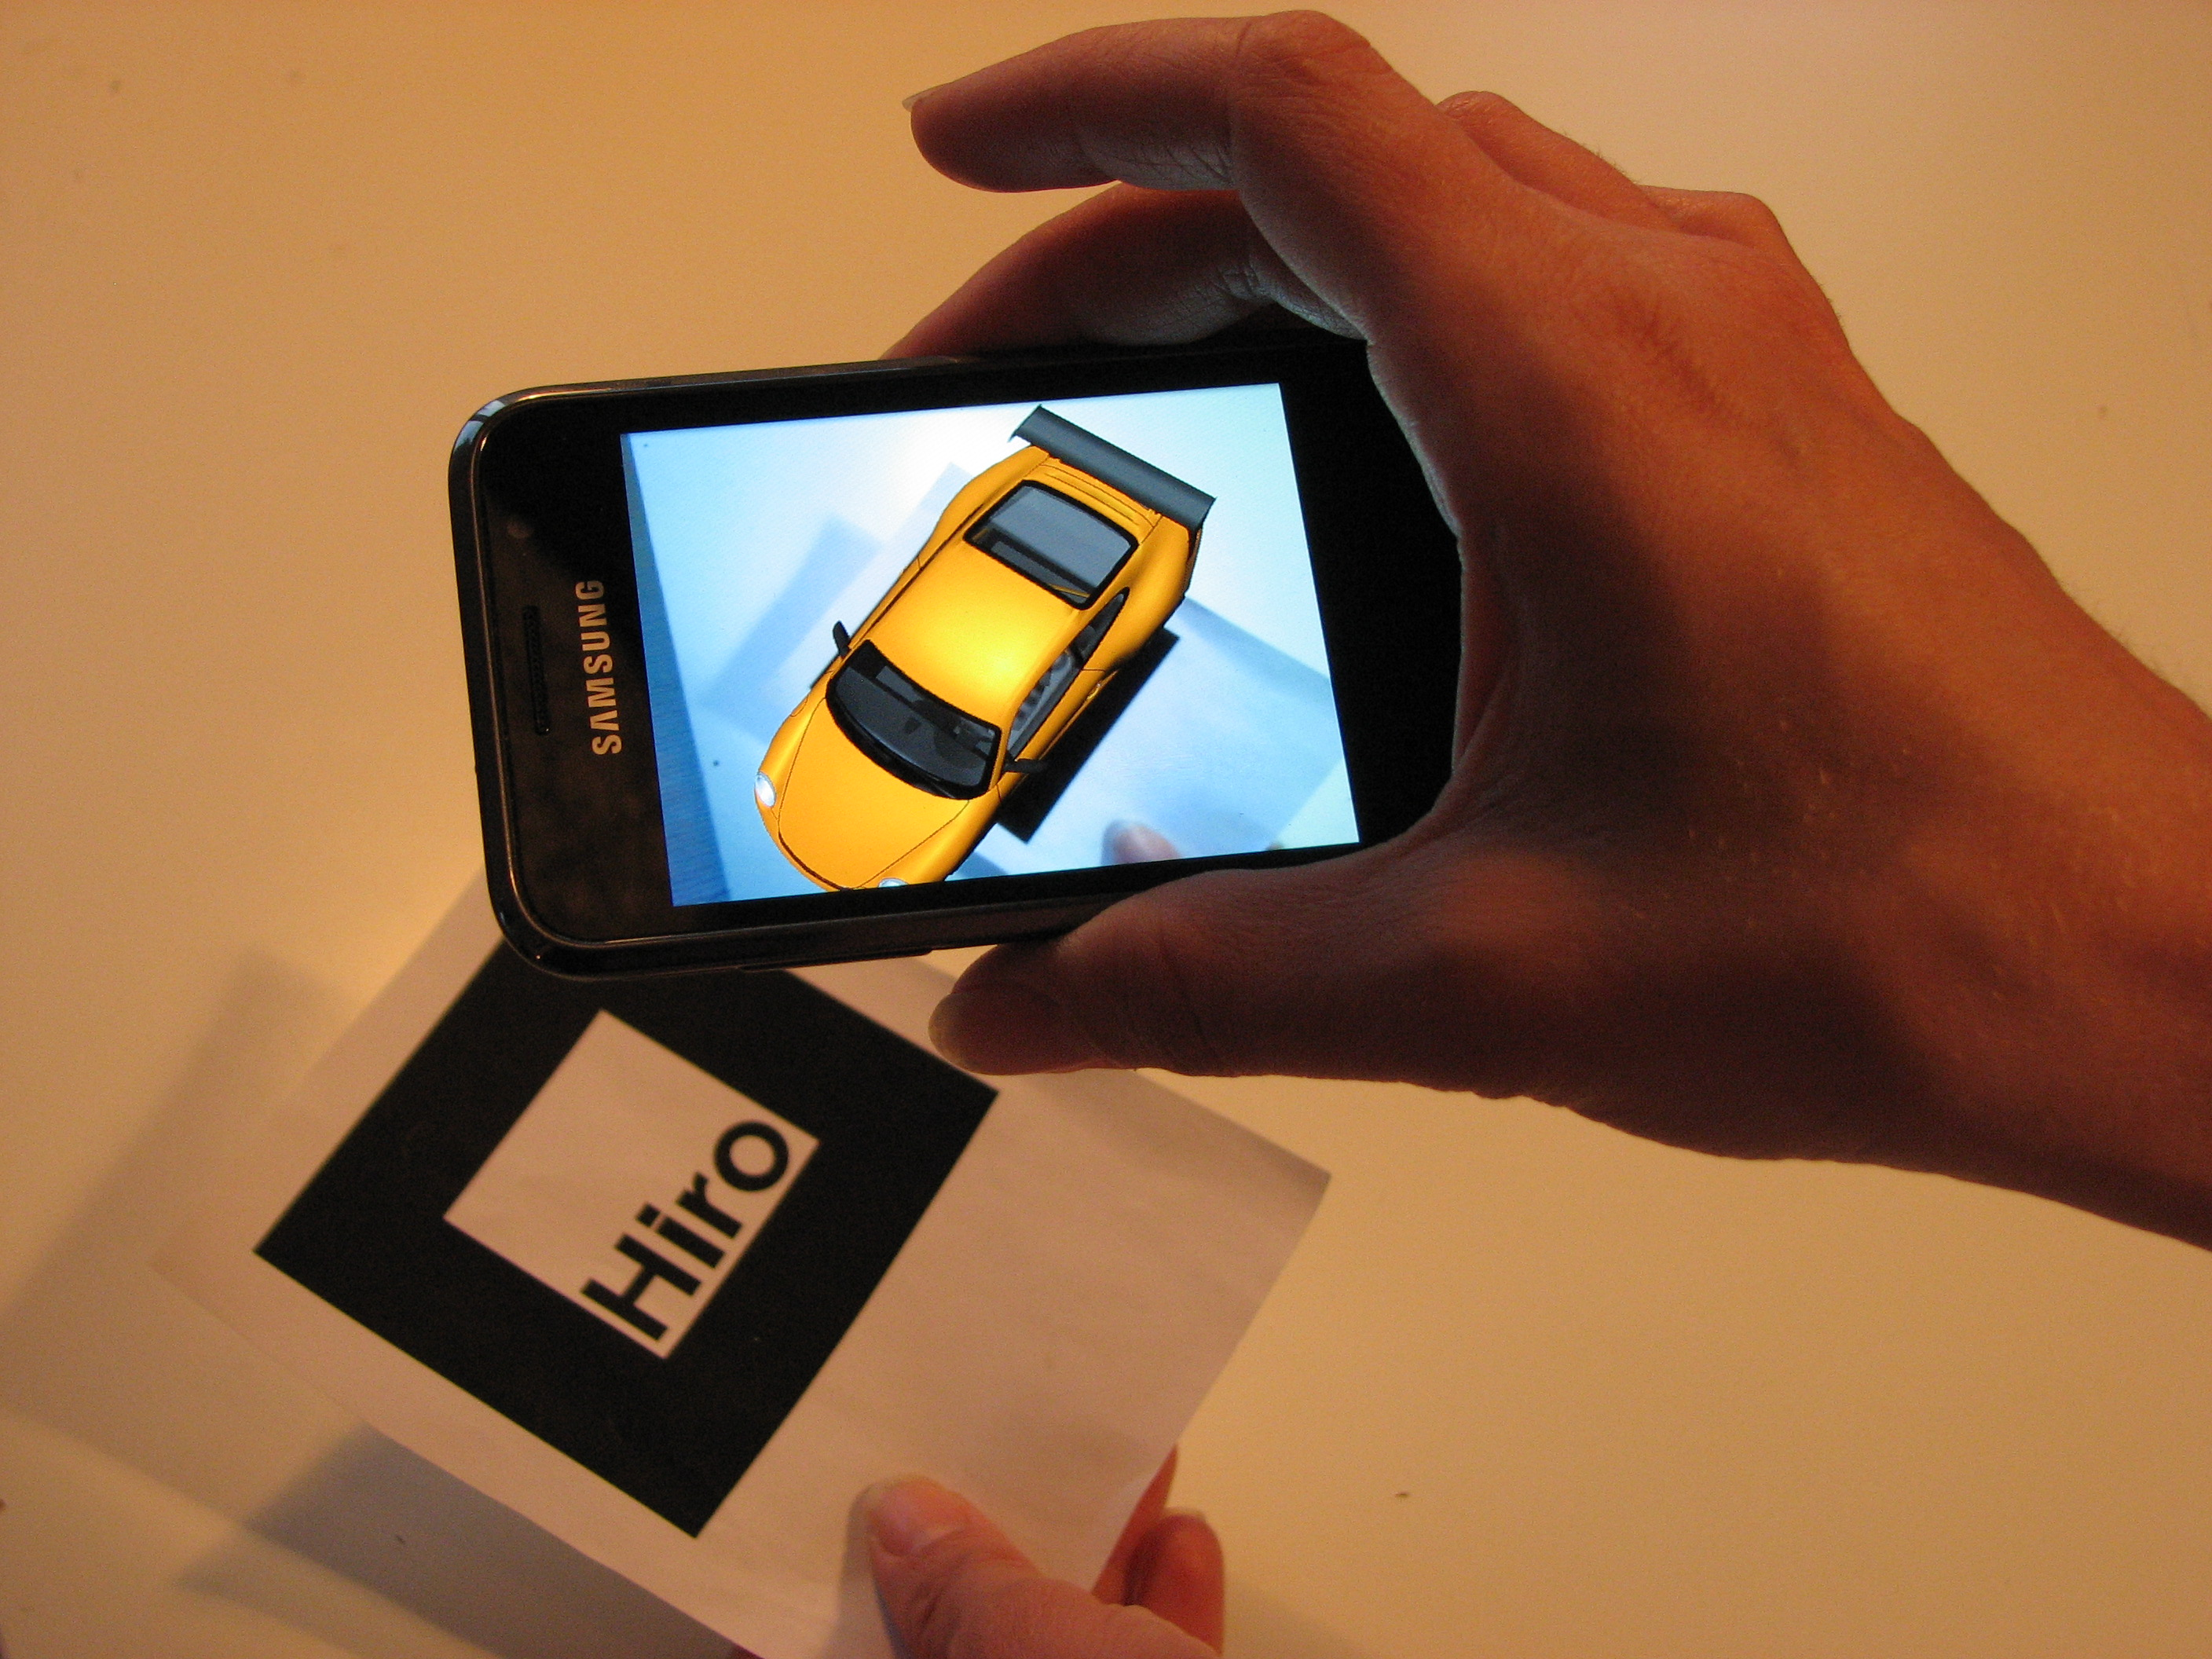
\includegraphics[width=0.9\textwidth]{images/artoolkit-demo.jpg}
\captionof{figure}{
Przykład zastosowania markera w ARToolkit
}
\small {źródło http://arblog.inglobetechnologies.com/?p=421}
\end{center}
\subsection{Przykład implementacji}
\paragraph{}
{\color{red}Opisać prefabrykaty}
\begin{center}
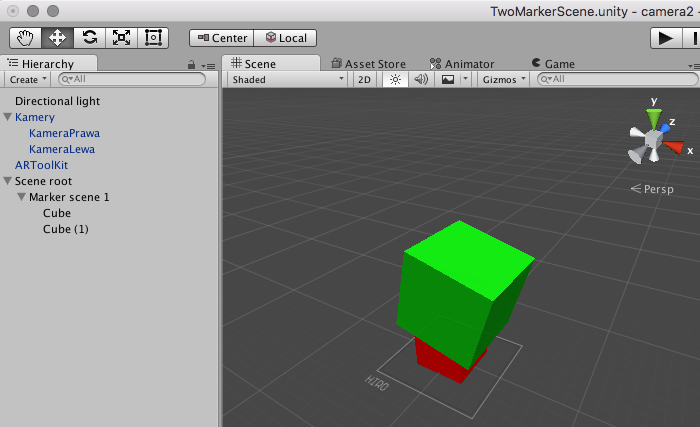
\includegraphics[width=0.9\textwidth]{images/artoolkit-przyklad.png}
\captionof{figure}{
Podstawowa impementacja
}
\small {źródło własne}
\end{center}
\subsection{Napotkane problemy i ograniczenia}
\paragraph{}
\begin{enumerate}
	\item Proces renderowania musi odbywać się na telefonie komórkowym, gdyż obraz kamery jest ciągle analizowany. Przy dużych scenach stworzonych w Unity moc obliczeniowa urządzenia jest niewystarczająca.
	\item Analizowanie pozycji markera przy nieustannie włączonej kamerze powoduje dużą drenację baterii urządzenia. Czas pracy na baterii jest mocno ograniczony
	\item Unity w wersji Personal (darmowej) skompilowanej pod platrformę mobilną (np. Android) nie udostępnia obsługi sieci (np. za pomocą połączenia TCP). Nie pozwala to na połączenie z zenętrznym kontrolerem.
	\item Sterowanie za pomocą kontrolera bez fizycznych przycisków z założonymi okularami Google Cardboard jest bardzo uciążliwe. W przyszłości należałoby rozważyć połączenie telefou z zewnętrznym kontrolerem typu PAD\footnote{https://pl.wikipedia.org/wiki/Gamepad}.
\end{enumerate}
{\color{red}Opisać}

\newpage
\section{Dalszy rozwój}

 
\newpage
\thispagestyle{empty}
 
  
\listoffigures
 
\listoftables

\lstlistoflistings


\begin{thebibliography}{99}
\bibitem{pa} Building Microservices,  Sam Newman , Wydanie 4, 2016
\end{thebibliography}

\end{document}
